\section{Preliminaries (2 pages)}

%\subsection*{Components}

We model autonomous systems as compositions of primitive components.
We superficially regard two kinds of components: rational components and irrational components.
Intuitively, only the behavior of the former can be finitely represented; the latter not.
Components cannot recognize themselves or others as being rational or irrational.
We use irrational components as primitives to model unpredictable environments.

\paragraph{Components}

Each component has a fixed number of ports.
A port can be thought of as a gateway, passing data in and out.
Components without ports are sealed and can no longer be composed.
Semantically, we define behavior of a component as a (non-well-founded) relation between ports.
Only rational components harbor a finite representation of its behavior.
See figure \ref{fig:Components} for a picture.
\begin{figure}[t]
\begin{centering}
\subfloat[\label{fig:Components}Components]{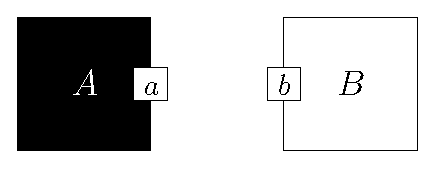
\includegraphics[scale=0.6]{pic/black-white-components}}$\qquad$\subfloat[\label{fig:Channels}Channels]{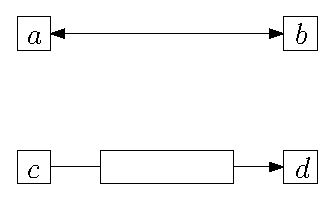
\includegraphics[scale=0.6]{pic/ports-channels}}$\qquad$\subfloat[\label{fig:Node}Node]{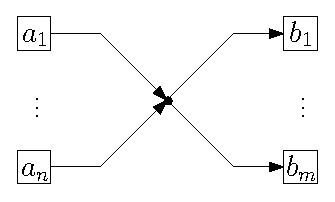
\includegraphics[scale=0.6]{pic/nodes}

}
\par\end{centering}
\caption{A black box is an irrational component; a white box is a rational
component. Channels are pictured by different edge styles. Nodes are
depicted by black dots, merging
incoming ports $a_1...a_n$ and replicating to outgoing ports $b_1...b_m$.}
\end{figure}

Studying ports is important.
One could stand\textemdash quite literally\textemdash next to a port and observe all data that is passed along.
Sometimes one observes no activity at all, which we denote by $*$.
Other times one observes a datum, which we leave uninterpreted.
Ports are characterized by the set of streams of its activity.
For example, we write $a=(*,d_{1},*,*,d_{2},\ldots)$ where $d_{1}$ is the first datum observed and $d_{2}$ is the second datum observed, and so on.

This work is based on Reo: a language for modeling agents as components.
The most important elements of this language are channels, nodes and compositions.
Channels and nodes are primitive components through which data \emph{flows} between ports.
We will later give two examples of the channels in figure \ref{fig:Channels}.
Nodes are used to link multiple channels together, see figure \ref{fig:Node}.
Finally, composition identifies the ports in complex constructions of channels and nodes.

\paragraph{Protocols}

We introduce protocols as a fundamental formalism for modeling systems.
Formal protocols are a generalization of formal languages,
in the sense that formal languages defines word membership,
and that formal protocols defines stream membership.
We now give some more details.

By $\Sigma$ we denote some countably infinite alphabet of symbols.
A finite sequence, or \emph{word}, is formed by juxtaposing symbols from $\Sigma$.
The set of all words is denoted $\Sigma^{*}$.
A formal language $\mathcal{L}$ is a subset of the set of all words,
i.e. $\mathcal{L}\subseteq\Sigma^{*}$.

An infinite sequence, or \emph{stream}, is formed by an infinite juxtaposing of symbols from $\Sigma$.
The set of all streams is denoted $\Sigma^{\omega}$.
A stream is isomorphic to a function $\sigma:\mathbb{N}\to\Sigma$,
and a $\sigma$ can be given by defining $\sigma(0)$ and the \emph{stream derivative} $\sigma'$.
Streams are informally described as infinite tuples,
in the shape $(x_{0},x_{1},x_{2},\ldots)$ where $x_i$ are elements of $\Sigma$.
A formal protocol $\mathcal{P}$ is a subset of the set of all streams,
i.e. $\mathcal{P}\subseteq\Sigma^{\omega}$.


\paragraph{Ports} Let $V$ denote a countably infinite set of port variables,
and let $D$ denote a set of data that contains some fixed constant $*\in D$.
The meaning of each datum $d\in D$ other than $*$ is application-specific.
By $D^{\omega}$ we mean a single stream of observations, called a \emph{data stream}.
Next, we consider a rational component $C$.
Let $V_{C}$ denote the finite set of port variables corresponding to $C$.
If $V_{C}$ is empty then the component is sealed.
Let $n=|V_{C}|$ be the number of ports of $C$.

We characterize the behavior of a rational component by a relation on data streams.
An $n$-ary relation $R$ on data streams can be seen as a set of tuples of data streams,
e.g. $(\sigma_{1},\sigma_{2},\ldots,\sigma_{n})\in R$.
We obtain the sets of data streams by projection:
we define $\sigma_i\in\Pi_i R$ if and only if $(\sigma_{1},\ldots,\sigma_i,\ldots,\sigma_{n})\in R$.
Equivalently, and more convenient for our purposes,
let $R$ be sets of streams of $n$-ary tuples of data.
That is, we let $R$ be a formal protocol with alphabet $\Sigma=D^{n}$.

Intuitively, one can compare our treatment to relational algebra,
where the attribute names of $n$-ary relations are our port variables.
By convention we identify a rational component $C$ and the relation specifying its behavior.
The ports $V_C$ are attributes of the $|V_C|$-ary relation.
We now characterize a port $v\in V_C$ by the set of data streams $\Pi_v C$.

\paragraph{Channels} We consider two channels: synchronous and asynchronous,
as depicted in figure \ref{fig:Channels} respectively on top and bottom.
Let $a$ and $b$ be two ports.
We specify the behavior of a synchronous channel between $a$ and $b$, denoted $S(a,b)\subseteq(D^2)^{\omega}$, as the largest relation such that:
$$\sigma\in S(a,b)\Leftrightarrow\left[\forall d\in D.\,\sigma(0)=(d,d)\right]\land\sigma'\in S(a,b)$$
that is, the two ports have equal data streams. We now specify the behavior of an asynchronous channel,
denoted $A(a,b)\subseteq(D^2)^{\omega}$, as the largest relation:
\begin{align*}
	\sigma\in A(a,b)\Leftrightarrow\forall d\in D.\, & \sigma(0)=(d,*)\,\land\\
	& \exists i.\,\sigma(i)=(*,d)\land\left[\forall j<i.\,\sigma(j)=(*,*)\right]\,\land\\
	& \phantom{\exists i.\,}\sigma^{(i+1)}\in A(a,b)
\end{align*}
where $\sigma^{(0)}=\sigma$ and $\sigma^{(n+1)}=\left(\sigma^{(n)}\right)'$ defines the repeated stream derivative.
Intuitively, an asynchronous channel is either inactive or passes a datum in a delayed fashion.
Let $i=0$ and see $\sigma(0)=(*,*)$.
If port $a$ offers a datum $d$ then port $b$  takes the same datum at some time later,
while both ports remain inactive in the mean time. Note that when $a$ and $b$ are also
connected by a synchronous channel, the behavior collapses into the singleton set accepting only $(*,*,\ldots)$.

\paragraph{Nodes}

Finally, we specify the node as depicted in \ref{fig:Node}.
Nodes have $n+m$ number of ports with $n,m\geq1$.
Its input ports are denoted $a^{\rightarrow}=a_1,\ldots,a_n$ and output ports $b^{\rightarrow}=b_1,\ldots,b_m$.
Note that by $\sigma(0)_i$ we denote the $i$-th projection of the initial element of
the stream $\sigma$ containing tuples $(a_1,\ldots,a_n,b_1,\ldots,b_m)$.
The behavior of nodes are characterized by the $(n+m)$-ary relation $N(a^{\rightarrow},b^{\rightarrow})$,
defined as the largest relation such that:
\begin{align*}
	\sigma\in N(a^{\rightarrow},b^{\rightarrow})\Leftrightarrow\, & \forall d\in D.\,
	\bigl[\exists i\leq n.\,\sigma(0)_i = d\land\left[\forall i'\leq n.\,i'\neq i\rightarrow\sigma(0)_{i'} = *\right]\\
	& \phantom{\forall d\in D.\, \bigl[}\forall j\leq m.\,\sigma(0)_{n+j}=d\bigr]\,\land\\
	& \sigma'\in N(a^{\rightarrow},b^{\rightarrow})
\end{align*}
where $i,i',j$ are non-zero.
Intuitively, nodes are synchronous channels that merge and replicate data.
Merge specifies that at most one of the $n$ channels can offer a datum,
and all others $n$ channels are inactive.
Replication specifies that all of the $m$ channels takes the datum offered.
Also, all ports of a node can be inactive.


\vfill
